\section{Additional proofs}
\label{sec:additional-proofs}

\begin{proof}[Proof of Theorem~\ref{thm:fixed_point}]
  Throughout the proof we abuse notation and denote the application
  of simplification rules to nodes and to elements of
  $\text{\lstinline{Set (Node, Ancestors)}}$ similarly, when no
  ambiguity arises.
%
  Consider the order $\leqSets$, defined on
  $\text{\lstinline{Set (Node, Ancestors)}} \times
  \text{\lstinline{Set (Node, Ancestors)}}$, as $S_1 \leqSets S_2$ if
  $|S_1| \leq |S_2|$ and there exists an injective map
  $\sigma : S_1 \rightarrow S_2$ s.t.\ $\sigma(N_1,A) = (N_2,A)$ with
  $N_2\subseteq N_1$.
  % 
  \begin{itemize}
  \item $\leqSets$ is a partial order. The proof that $\leqSets$ is
    reflexive and transitive is straightforward.  To prove that it is
    antisymmetric, assume that $S_1\leqSets S_2$ and
    $S_2 \leqSets S_1$.  This means that $|S_1|=|S_2|$ and,
    furthermore, the maps $\sigma_1 : S_1 \rightarrow S_2$ and
    $\sigma_2 : S_2 \rightarrow S_1$ are bijective. Notice that
    $\sigma_1\circ \sigma_2$ is the identity map, otherwise we could
    consider $(N,A)\in S_2$ where $N$ is minimal w.r.t.\ inclusion and
    s.t.\ $(\sigma_1\circ \sigma_2)(N,A) \neq (N,A)$, i.e.,
    $(\sigma_1\circ \sigma_2)(N,A) = (N',A)$ with $N'\subseteq N$ for
    some $(N',A)\in S_2$; due to the minimality of $N$, we would have
    $(\sigma_1\circ \sigma_2)(N',A) = (N',A)$, which would contradict
    the injectivity of $\sigma_1\circ \sigma_2$. Since
    $\sigma_1 (N,A) = (N',A)$ is such that $N'\subseteq N$, we shall
    have $\sigma_1 (N,A) = (N,A)$. Hence, $S_1=S_2$.
  \item The simplification function is order-preserving.
	To prove that the reflexive rule preserves the order, let
        $S_1$ and $S_2$ be s.t.\ $S_1\leqSets S_2$ and let us prove
        that
        $\text{\lstinline{reflex}}
        S_1\leqSets\text{\lstinline{reflex}}S_2$.
	% Start noticing that $|S| = |\text{\lstinline{reflex}} S|$,
	% hence
	% the number of children nodes is preserved by using the
	% reflexive
	% rule, let us analyze each case.
	Let $(N,A)\in \text{\lstinline{reflex}} S_1$ and notice that
        there exists $(N_1,A)\in S_1$, such that
        $\text{\lstinline{reflex}} N_1 = N $, and so, in $S_2$ there
        is $(N_2,A)=\sigma(N_1,A)$ s.t. $N_2\subseteq N_1$.  Since
        $N_2\subseteq N_1$, we have
        $\text{\lstinline{reflex}} N_2 \subseteq
        \text{\lstinline{reflex}} N_1 = N$.  The same reasoning
        applies to prove that if $S_1\leqSets S_2$ then
        $\text{\lstinline{congruence} }
        S_1\leqSets\text{\lstinline{congruence} }S_2$.
%
	To prove that \lstinline{bpa1} preserves the order,
	note that 
	$S \subseteq \text{\lstinline{bpa1} }S$. Assume that 
	$S_1\leqSets S_2$, let $(N,A)\in \text{\lstinline{bpa1} }S_1$, 
	and denote by $(N_1,A)\in S_1$ and $(\vec X,\vec Y)\in N_1$  
	the node and the pair whose simplification 
	led to $(N,A)$. We know that exists $(N_2,A)\in S_2$
	s.t.\ $N_2 \subseteq N_1$. If $(\vec X,\vec Y)\in N_2$,
	then the \lstinline{bpa1} simplification of $N_2$ with
	the pair $(\vec X,\vec Y)$ generates 
	$(N',A)\in \text{\lstinline{bpa1} }S_2$ such that 
	$N'\subseteq N$. On the other hand, if 
	$(\vec X,\vec Y)\not \in N_2$, then $N_2\subseteq N$ 
	and, since  $S_2 \subseteq \text{\lstinline{bpa1} }S_2$,
	$(N_2,A)\in \text{\lstinline{bpa1} }S_2$ is such that
	$N_2\subseteq N$.
	The same reasoning applies to \lstinline{bpa2}. 
      \end{itemize}
      
      Having proved that each simplification function preserves the
      order, and since the simplification procedure results from the
      successive application of these rules, we have proved that the
      simplification function also preserves the order.\smallskip
      %
      \begin{itemize}
      \item $(\text{\lstinline{Set (Node, Ancestors)}}, \leqSets)$ is
        a lattice. Given
        $S_1, S_2\in \text{\lstinline{Set (Node, Ancestors)}}$,
        $S_1 \cup S_2$ is an upper bound and $S_1 \cap S_2$ is a lower
        bound for $S_1$ and $S_2$.
      \item $(\text{\lstinline{Set (Node, Ancestors)}}, \leqSets)$ is
        a complete lattice. Given
      $\mathcal{B}\subseteq \text{\lstinline{Set (Node, Ancestors)}}$:
      $\bigcup_{S\in \mathcal{B}} S$ is an upper bound and
      $\bigcap_{S\in \mathcal{B}} S$ is a lower bound for the sets in
      $\mathcal{B}$.
    \end{itemize}
    Using Tarski's fixed point theorem~\cite{tarski1955lattice}, we
    conclude that the simplification function has a fixed point in
    $\text{\lstinline{Set (Node, Ancestors)}}$.
\end{proof}


% \section{Application}
	
% 	We use this additional section to address the details of Example~\ref{ex:example1}.
	
% \begin{example}[Detailed analysis of Example~\ref{ex:example1}]
% 	Let the base types $\intk$ and $\boolk$ represent integer and Boolean values, $\ell$ and $m$ denote labels for the internal and external choices on the branches, and consider the types:
% 	\[
% 	S\triangleq \mu x. (\oplus\{\ell\colon !\,\intk; \&\{\ell\colon x, m\colon \skipk \} , m\colon !\, \boolk; \&\{\ell\colon x, m\colon \skipk \} \}); \mu x. (\&\{\ell\colon\skipk, m\colon ?\,\boolk; x \})
% 	\]
% 	\[
% 	T\triangleq \mu x. (\oplus\{\ell\colon !\,\intk , m\colon !\, \boolk\}; \&\{\ell\colon x, m\colon \mu y. (\&\{\ell\colon\skipk, m\colon ?\,\boolk; y \})\})
% 	\]
% 	$S$ and $T$ can be represented as PA graphs as depicted on Figure~\ref{fig:PAgraphsST}.
	
% 	\begin{figure}[h!]
% 		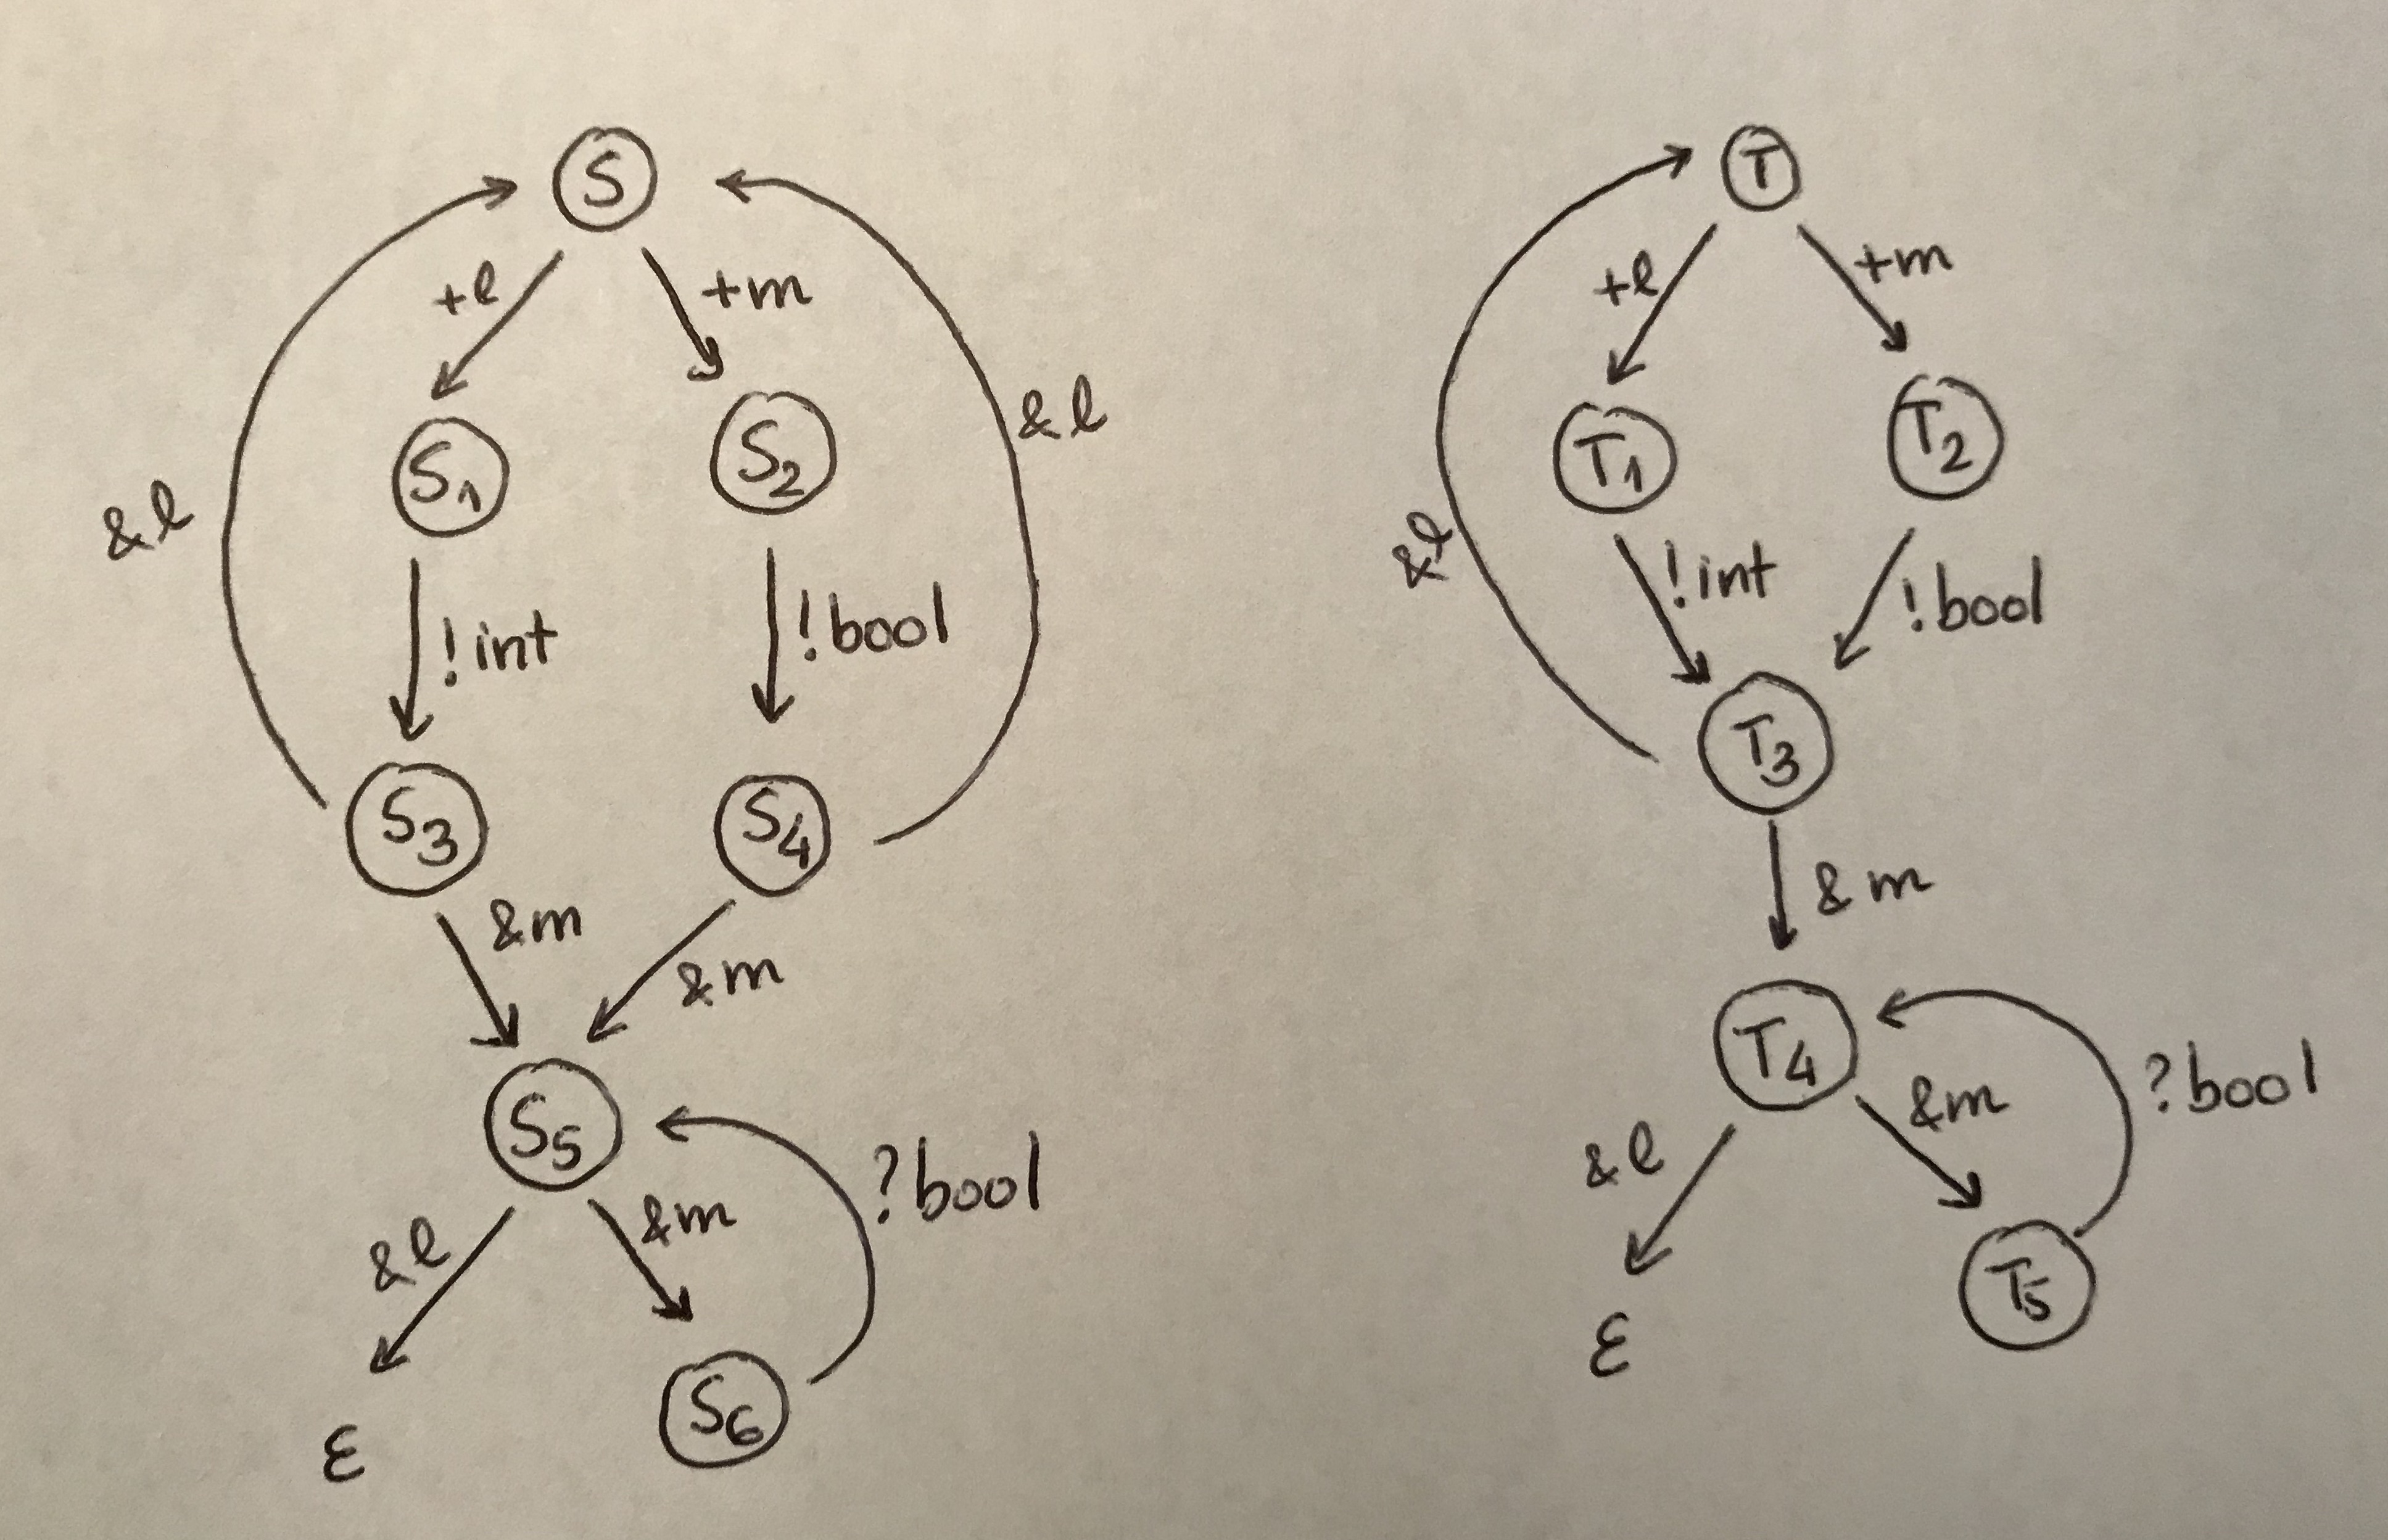
\includegraphics[width=\columnwidth]{PAgraphsST.jpg}
% 		\caption{Process algebra graphs for $S$ and $T$.}
% 			\label{fig:PAgraphsST}
% 	\end{figure}
% 	The algorithm we propose in this work derives the expansion tree for $S\sim T$ as a sequence of nodes. The nodes in this expansion tree can be labeled with a trace of the nodes that lie ahead, based on the syntactical structure of $S$ and $T$. We get the following sequence of labeled nodes in the expansion tree for $S\sim T$:\\\\
% \begin{tikzcd}[cells={nodes={draw=black}}, column sep=large]
%   \enspace (S,T) \enspace \ar[r,"expand"]
% & \enspace  (S_1S_3S_5,T_1T_3), (S_2S_4S_5, T_2T_3) \enspace \ar[r,"expand"]
% & \enspace  (S_3S_5,T_3), (S_4S_5, T_3) \enspace  
% \end{tikzcd} 
% $\xrightarrow{\text{expand}}$\\\\
% \begin{tikzcd}[cells={nodes={draw=black}}, column sep=large]
% & \enspace(SS_5,T),(SS_5,T),(S_5,T_4),(S_5,T_4)  \enspace\ar[r,dashed,"bpa1"]
% &\enspace (S_5,\varepsilon),(S_5,T_4) \enspace 
% \end{tikzcd} 
% $\xrightarrow{\text{expand}}$ \\\\
% \begin{tikzcd}[cells={nodes={draw=black}}, column sep=large]
% &\enspace (S_6S_5,T_5T_4), (\varepsilon,\varepsilon) \enspace \ar[r,dashed,"reflex"] 
% &\enspace (S_6S_5,T_5T_4)\enspace \ar[r,"expand"]
% & \enspace(S_5,T_4)\enspace \ar[r,dashed,"bpa1"]
% &\emptyset\\
% \end{tikzcd}

% 	The process alternates between simplification and expansion operations, denoted by dashed and solid arrows, respectively. Having reached an empty node, we conclude that $S\sim T$.\\\smallskip
	
% 	Now consider the types:
% 	\[ R \triangleq \mu x.\&\{\ell\colon ?\,\boolk;x, m\colon ?\,\intk;x;x \} \text{ and }  U \triangleq \mu x.\&\{\ell\colon ?\,\boolk, m\colon ?\,\intk;x;x\} \enspace .\]
	
% 	$R$ and $U$ are represented as PA graphs as shown in Figure~\ref{fig:PAgraphsRU}.
	
% 	\begin{figure}[h!]
% 	\centering
% 		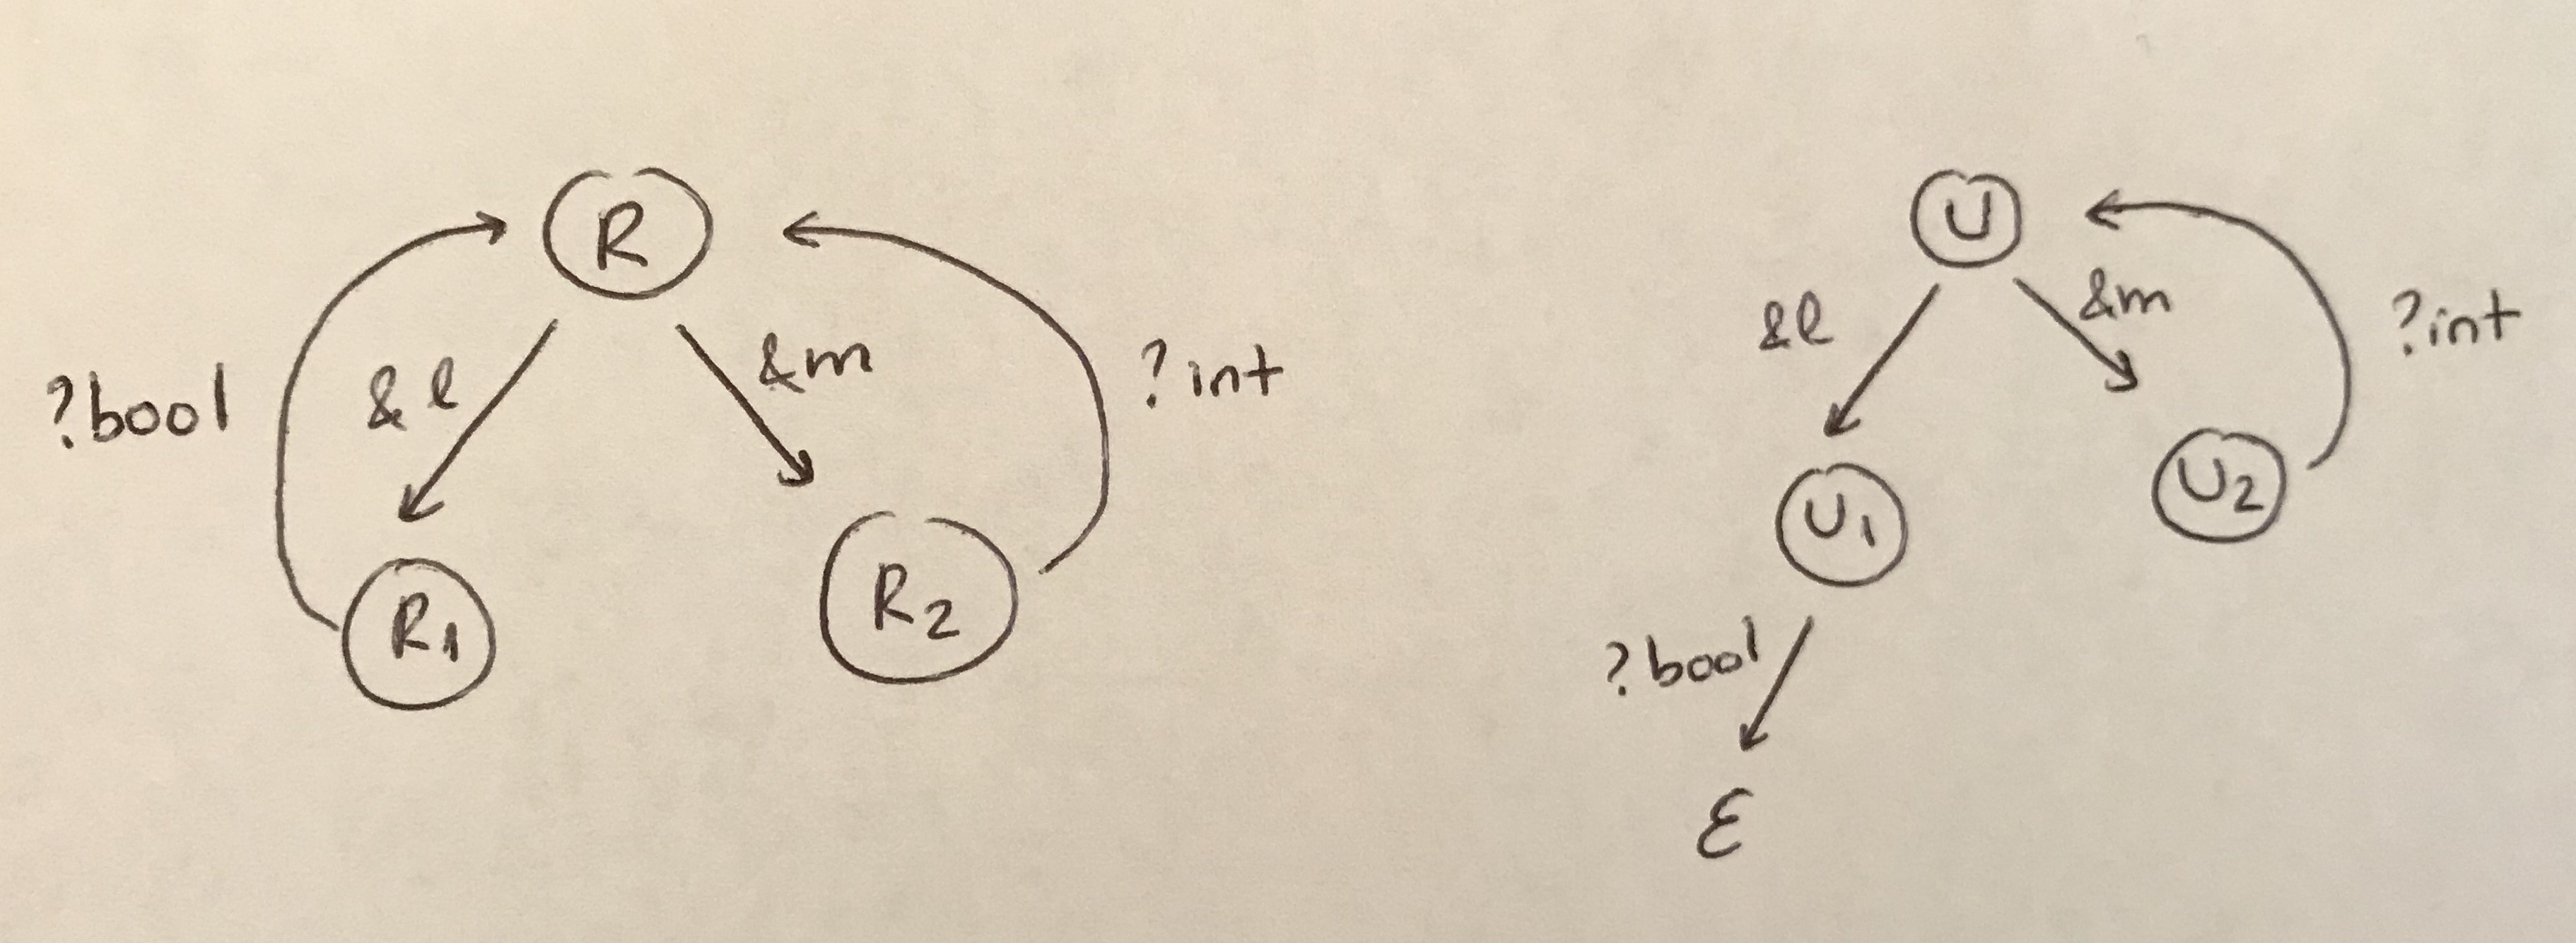
\includegraphics[width=14cm]{PAgraphsRU.jpg}
% 		\caption{Process algebra graphs for $R$ and $U$.}
% 		\label{fig:PAgraphsRU}
% 	\end{figure}
% 	Using the porposed algorithm, we get the following expansion list build upon the syntactical structure of $R$ and $U$ and their representations as PA graphs:\\\\
% \begin{tikzcd}[cells={nodes={draw=black}}, column sep=large]
%   (R,U) \ar[r,"expand"]
% & (R_1 R,U_1), (R_2 R R, U_2 U U) \ar[r,"expand"]
% & (R,\varepsilon), (RR, UU) \ar[r,dashed,"bpa1"] 
% & (R,\varepsilon), (U,\varepsilon) 
% \end{tikzcd} 
% \enspace  $\times$\\\\
% We notice that the last step results from applying BPA1 rule~\cite{janvcar1999techniques} to $(RR,UU)$ knowing that $(R,U)$ is an ancestor node, which leads to the pairs $(R,\varepsilon)$ and $(U,\varepsilon)$. As we then fail to obtain new derived nodes, we decide the type equivalence negatively and conclude that $R\not\sim U$.
% 	\hfill $\triangle$
% \end{example}


%%% Local Variables:
%%% mode: latex
%%% TeX-master: "main"
%%% End:
